\documentclass[11pt, a4paper]{book}
\usepackage{parskip}
\usepackage[top=1.5cm, left=1cm, right=1cm, bottom=2.5cm]{geometry}
\usepackage{fontspec}
\usepackage{graphicx}
\setmainfont{DejaVu Serif}
\begin{document}
\chapter{Android IPC Mechanism}
\section{Overview}
IPC = Inter-process Communication. The IPC in android is Binder, a lightweiget
RPC(Remote Procedure Communication) mechanism.

To solve to background problems: Applications and services may run in separate
processes but must communicate and share data, IPC can introduce significant
processing overhead and security hold.

\paragraph{IPC Abstraction}
\begin{description}
    \item [Intent] The highest level abstraction
    \item [AIDL] Android Interface Definition Language, inter process method
        invocation.
    \item [Binder] Kernel driver
    \item [ashmem] shared memory.
\end{description}
\begin{figure}
    \centering
    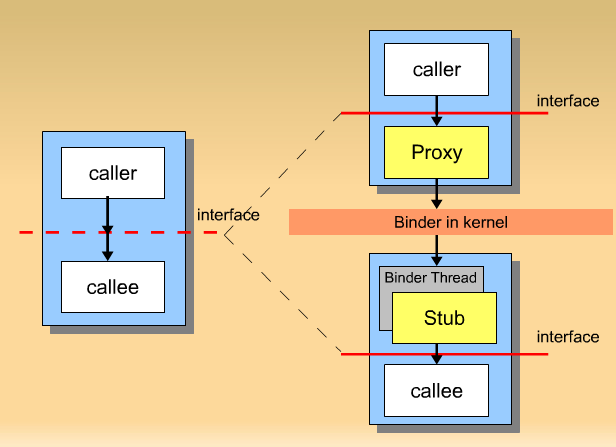
\includegraphics[scale=0.5]{IPC_invo.png}
    \caption{Innovation of android IPC}
\end{figure}


\section{Intent:simple low level}
Intent: The highest level abstraction IPC in Android. Requests are queued and
handled sequentially.

The android system uses Intent object to enable applications to specify an
Activity or Service. Intent objects also deliver data from one app to another.

It's loosely coupling: The sender need not choose the receiver, the sender can
specify "action". Then proper receiver is chosen and handles it.
\section{AIDL and Remote Methods}
The overall structure of android IPC system consists of four major block, one in
kernel space, and the other three in use space. The overall structure is shown
in the diagram below:
\begin{figure}
    \centering
    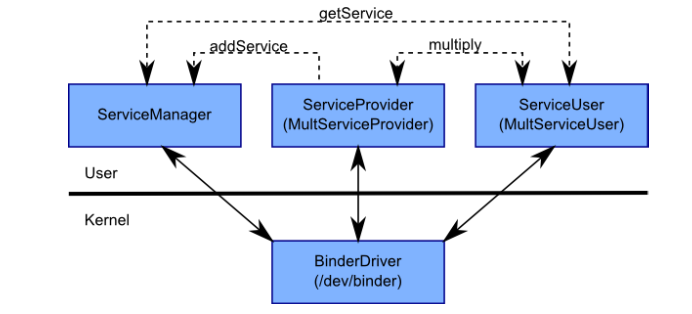
\includegraphics[scale=0.5]{IPC_structure.png}
    \caption{Overall architecture of the Android IPC system}
\end{figure}
\begin{itemize}
    \item \verb|BinderDriver|: the core of IPC system. It \textbf{passes data} between a
        ServiceProvider and a ServiceUser. This kernel component is provide by
        Android.
    \item \verb|ServiceProvider|: Provides some kind of service. It \textbf{parses the
        received RPC data} from the BinderDriver and \textbf{does the real
        work}.
    \item \verb|ServiceManager|: This is a special singleton ServiceProvider
        that \textbf{provides service manager services} for other service providers.
    \item \verb|ServiceUser|: This is the client. It \emph{remote calls the
        ServiceProvider by generating an RPC} and sending it to the
        BinderDriver. Application developer typically write their own
        ServiceUser as part of their application.

\end{itemize}
The typical flow of events for fictitious MultServiceProvider(a service provider
that multiplies two number for a client.) and a MultServiceUser client which
doesn't know how to multiplication and needs to use the MulServiceProvider.
\begin{enumerate}
    \item ServiceManager Runs first and registers a special node(Node O) with the 
        BinderDriver;
    \item The MultiServiceProvider gets an IServiceManager proxy object for the special node 0 by calling the global 
        \verb|defaultServiceManager()|function 
    \item The MultServiceProvider then calls
        \begin{verbatim}
        defaultServiceManager()->addService("Multiplier", new MultServiceProvider())
        \end{verbatim}
        to add itself as a serviceprovider and then
        waits in an infinite loop for someone to request its services. The
        addService RPC call is routed to the ServiceManager through 
        BinderDriver.
    \item The BinderDriver notices that the RPC to the ServiceManger it
    generates another service, so besides routing the RPC to the ServiceManager
    it generates another node (let's call it node M), for the new
    MultServiceProvider.
    \item The ServiceManager reads the data from the BinderDriver and processes
        the \verb|IServiceManager::addService| RPC call.
    \item The MultServiceUser client process gets a IServerManager proxy object
    for the special node O. (again by using defultServiceManger).
    \item The client dose an IServiceManager::getService("Multiplier")RPC call
    to get the MultServiceProvider. This call is routed to the ServiceManager
    through the BinderDriver.
    \item The ServiceManager reads the RPC data from the BinderDriver, processes
    the IServiceManager::getService requestand returns back the node
    representing the MultServiceProvider.
    \item MultServiceUser calls MultServiceProvider::multiply(a,b). This call is
    routed to MultServiceProvider by the BinderDriver.
    \item The MultServiceProvider handles the MultServiceProvider::multiply RPC
    call and sends the product of 2 number in a reply to BinderDriver.
    \item The BinderDriver routes the reply back to the client.
    \item The client reads the data from BinderDriver contains the product.
\end{enumerate}
\section{Using Android IPC binders from native code}
When executed with an integer argument (ex: "binder 743"), the binary acts as a
\textbf{client} that searches for the "Demo" service, binds to it, and exercises
its API.

The suggested way to run this demo to have 3 window open and issue the following
commands in them:
\begin{enumerate}
    \item \verb|adb logcat -v time binder_demo:* *:S|
    \item \verb|adb shell binder|
    \item \verb|adb shell binder 456|
\end{enumerate}

We start by defining an interface (think AIDL) that will be \emph{shared between the
service and client}:
\begin{verbatim}
class IDemo : public IInterface {
    public:
        enum {
            ALERT = IBinder::FIRST_CALL_TRANSACTION,
            PUSH,
            ADD
        };
        // Sends a user-provided value to the service
        virtual void        push(int32_t data)          = 0;
        // Sends a fixed alert string to the service
        virtual void        alert()                     = 0;
        // Requests the service to perform an addition and return the result
        virtual int32_t     add(int32_t v1, int32_t v2) = 0;
 
        DECLARE_META_INTERFACE(Demo);
};
 
// This implementation macro would normally go in a cpp file
IMPLEMENT_META_INTERFACE(Demo, "Demo");
\end{verbatim}

Next we define the \textbf{server end}, which is made up of 2 classes:BnDemo,
and its derived class, Demo.

BnDemo extracts the argument from the data Parcel sent by the client, calls the
appropriate virtual function(implemented in the Demo class) to do the
heavy-lifting, and packs the returned values into the reply Parcel to be sent
back to the client.
\begin{verbatim}
//Extract the data
class BnDemo : public BnInterface<IDemo> {
    virtual status_t onTransact(uint32_t code, const Parcel& data,
                                Parcel* reply, uint32_t flags = 0);
};

status_t BnDemo::onTransact(uint32_t code, const Parcel& data,
                            Parcel* reply, uint32_t flags) {

    data.checkInterface(this);

    switch(code) {
        case ALERT: {
            alert();
            return NO_ERROR;
        } break;
        case PUSH: {
            int32_t inData = data.readInt32();
            push(inData);
            return NO_ERROR;
        } break;
        case ADD: {
            int32_t inV1 = data.readInt32();
            int32_t inV2 = data.readInt32();
            int32_t sum = add(inV1, inV2);
            reply->writeInt32(sum);
            return NO_ERROR;
        } break;
        default:
            return BBinder::onTransact(code, data, reply, flags);
    }
}
\end{verbatim}

This is the Demo class, which would normally do the real work on the service
side of the binder:
\begin{verbatim}
class Demo : public BnDemo {
    virtual void push(int32_t data) {
        // Do something with the data the client pushed
    }
    virtual void alert() {
        // Handle the alert
    }
    virtual int32_t add(int32_t v1, int32_t v2) {
        return v1 + v2;
    }
};
\end{verbatim}

Now we define a service proxy, to be used on the client side. Notice again that
any data the client needs to send to the service is packed in Parcel and results
are also returned in a Parcel.

\begin{verbatim}
class BpDemo : public BpInterface<IDemo> {
    public:
        BpDemo(const sp<IBinder>& impl) : BpInterface<IDemo>(impl) { }

        virtual void push(int32_t push_data) {
            Parcel data, reply;
            data.writeInterfaceToken(IDemo::getInterfaceDescriptor());
            data.writeInt32(push_data);
            remote()->transact(PUSH, data, &reply);
        }

        virtual void alert() {
            Parcel data, reply;
            data.writeInterfaceToken(IDemo::getInterfaceDescriptor());
            remote()->transact(ALERT, data, &reply, IBinder::FLAG_ONEWAY);
        }

        virtual int32_t add(int32_t v1, int32_t v2) {
            Parcel data, reply;
            data.writeInterfaceToken(IDemo::getInterfaceDescriptor());
            data.writeInt32(v1);
            data.writeInt32(v2);
            remote()->transact(ADD, data, &reply);

            int32_t res;
            status_t status = reply.readInt32(&res);
            return res;
        }
};
\end{verbatim}
Finally, we start the service as follows:
\begin{verbatim}
defaultServiceManager()->addService(String16("Demo"), new Demo());
android::ProcessState::self()->startThreadPool();
\end{verbatim}

And the client can now connect to the service and call some of the provided
function:
\begin{verbatim}
sp<IServiceManager> sm = defaultServiceManager();
sp<IBinder> binder = sm->getService(String16("Demo"));
sp<IDemo> demo = interface_cast<IDemo>(binder);
 
demo->alert();
demo->push(65);
int32_t sum = demo->add(453, 827);
\end{verbatim}
Note that Binder Server is basically an object of Binder class. When the object
is created, it will start a new process internally listening to the Message from
Binder Driver. When receiving message, it will receive the 
\section{Implementation with Java android code}
\subsection{Remote Methods and AIDL}
Three steps to create and use remote methods in Android:
\begin{enumerate}
    \item Define the interface in AIDL
    \item Implement the interface. That is write methods that match the
        signatures in the interface and that perform the operations you want in
        the program that provides the desired services.
    \item Invoke the method where you want to use them.
\end{enumerate}
\subsection{Android Interface Definition Language}
To communicate from one process to another, data store in memory has to be moved
across process boundaries. That means the data has to be packaged for
transport(Marshalled) and put into the right member variables after the data has
been moved across the process boundary.(Unmarshalled)

Usually, marshalling and unmarshelling data is performed the parameters in a
remote method call, to let you pass data from one application to another and
return results.

Marshalling and unmarshelling data is tedious, so usually use an
\textbf{interface} definition language that generates calls to marshalling
methods. The syntax of the interface definition language \emph{resembles the
main language in use}, so that a remote procedure call closely resembles a
normal method call. 

AIDL syntax is identical to Java interface definition syntax, except that in
AIDL you can label the parameters for remote method calls as in, out or inout. 

Parameter labeled in will be transferred to the remote method, out will be
returned to the caller from the remote method. Example:
\begin{verbatim}
interface ISecondary {
    /**
     * Request the PID of this service, to do evil things with it.
     */
    int getPid();

    /**
     * This demonstrates the basic types that you can use as parameters
     * and return values in AIDL.
     */
    void basicTypes(int anInt, long aLong, boolean aBoolean, float aFloat,
            double aDouble, String aString);
}
\end{verbatim}

The ADK for Eclipse automatically compiles AIDL to java, and the generated java
code do a bunch of things.

Now let's take a look at the \verb|android.os.IInterface| class, its a base type
on which all the interfaces created by AIDL are built, so they can be referenced
through references of the same type. \verb|ISecondary extends IInterface|

Most of the code in ISecondary interface is part of the definion of an abstract
class called \verb|Stub| class.

The word "stub" was chosen to refer to this class because remote method systems work by creating a method on the client with the same name as the method that runs on the server. The client method is considered a "stub" because it doesn't actually carry out the operation requested; it just marshalls the data, sends it to the server, and unmarshalls the return value. We'll show some details later in this chapter.

\subsection{Implementing the Stub interface}
The first line extends the abstract class and make a new instance of it:
\begin{verbatim}
private final ISecondary.Stub mSecondaryBinder = new ISecondary.Stub() {
    public int getPid() {
        return Process.myPid();
    }
    public void basicTypes(int anInt, long aLong, boolean aBoolean,
            float aFloat, double aDouble, String aString) {
    }
};
\end{verbatim}
This is all you need to do to turn a method in your application to a remote
method. The rest of the work of invoking the method in the other application

So, for a remote interface generated by AIDL, the code takes the abstract Stub class and implements the method code that will actually be used. But how does data from another process get to these methods? That is where the onTransact method comes in.

The \verb|onTransact| method is called \emph{when data in a Parcel object is
delivered to a remote interface in an Android program}. This method is generated
by AIDL for each remote interface. In this case, it reads each argument to the
method from Parcel object, makes the method call, and writes the result to
another Parcel object used for the return value of remote method.
\subsection{Getting an instance of the remote Proxy object}
There is one more part to this story: how does a different application find out
aobut the interface called ISecondary, and how does the caller of the remote
method actually call these methodsd? 

Answer: the asInterface method of Stub class, and the Proxy class nested within
Stub.

And that means that any application that wants to make a remote method call must
share the interface definition with the application that implements the
interface.

In practice terms, that means that the calling application and the application
that implements the remote interface have to be compiled with the same AIDL
files.

Now let's take a look at how the remote interface gets called. In the ApiDemo
code we are using as an example here, this happens in the RemoteServiceBinding
class, where the asInterface method is called:
\begin{verbatim}
mSecondaryService = ISecondary.Stub.asInterface(service);
\end{verbatim}

The parameter named service here is a reference to an IBinder interface. The Binder abstract class implements IBinder, and the Stub class (the guts of what AIDL has generated) extends Binder. Let's see how this parameter is used in the asInterface method:
\begin{verbatim}
public static com.example.android.apis.app.ISecondary asInterface(android.os.IBinder 
  obj) {
    if ((obj == null)) {
        return null;
    }
    android.os.IInterface iin = (android.os.IInterface) 
      obj.queryLocalInterface(DESCRIPTOR);
    if (((iin != null) && (iin instanceof com.example.android.apis.app.ISecondary))) {
        return ((com.example.android.apis.app.ISecondary) iin);
    }
    return new com.example.android.apis.app.ISecondary.Stub.Proxy(obj);
}
\end{verbatim}

Here the parameter is named obj, and first it is tested to see whether it is null. Then, asInterface checks to see whether there is an instance of ISecondary with the correct name. What that means is that the "remote" interface we were looking for is actually in the same application as the code calling it. And that means no inter-process communication is necessary. Otherwise, if it isn't a local interface, an instance of the Proxy object is created. Remember that this code is executing in the context of the application that wants to call the remote interface.

\verb|asInterface| make use of the \verb|querylocalinterface()| method, to
provide a consistent interface for remote client and the local calling.

Looking inside the Proxy class, we see that it has methods that have the same signature as the remote methods defined in the AIDL file. Here, unlike in the abstract class Stub, the methods are implemented, and the implementations create Parcel objects and fill them with the "flattened" parameters in exactly the right order for the onTransact method to "unflatten" them and call the remote methods.

That means an application calls a remote method by getting an instance of the Proxy class and calling the remote methods as if they were local. You can see this here, excerpted from the RemoteServiceBinding class:
\begin{verbatim}
int pid = mSecondaryService.getPid();
\end{verbatim}

Recall that mSecondaryService is returned from the ISecondary.Stub.asInterface method. Because the caller gets a Proxy object and the remote methods are implemented in a Stub object, and because both Proxy and Stub implement ISecondary, it all looks like a local method call, but the implementations of the methods are completely different in the calling application and the application that implements the remote methods.

In summary:
\begin{itemize}
    \item You define remote interfaces in AIDL
    \item AIDL turns your remote interface definition into a java
        interface with \verb|Stub| and \verb|proxy| classes nested
        inside.
    \item Both the application that \emph{calls the remote method} and the
        application that \emph{implements it} use the same AIDL file and the
        same generated interface.
\end{itemize}
The application calling the remote interface gets an instance of the Proxy class
that implements the very same interface it is defined inside of. They package up
their parameters into a Parcel object and send them to the application that
implements the remote methods and unpackages and returns the results.

In the remote application, a concrete class extend Stub has implementations of
the remote methods. The onTransact method "unflatten" data in a Parcel object,
calls the remote methods and "flattens" the result.

\subsubsection{Publishing an interface}
The server publishes an interface to \emph{make it possible for other activities
to find it} Publishing is accomplished by overriding the onBind method of
Service class.

The client calls the bindService method of the Context class, calling a call to
the server's onBind method. The bindService an onBind methods are the
"handshake" required to start using a remote interface in a specific Service
object in a specific process running in the Android environment. 
\begin{figure}
    \centering
    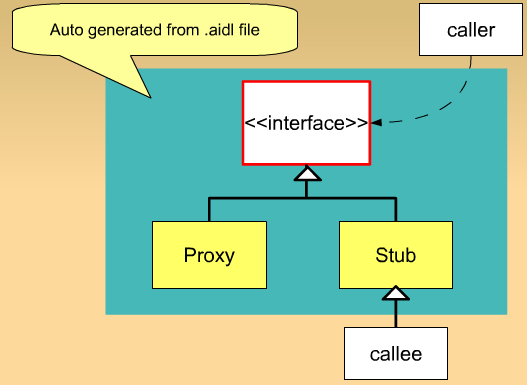
\includegraphics[scale=0.5]{AIDL.png}
    \caption{AIDL}
\end{figure}
\subsection{Dive into the mechanism}
The binder framework is actually works without a proxy. The basic the procedure
is:
\begin{itemize}
    \item To define a Binder Server, we subclass the Binder class and
        override the onTransact method.
    \item At the creation of Binder Server, a new thread and a mRemote
        object, which is also the subclass of Binder will be created.
    \item mRemote override the transact method.
    \item To actually call the remote method, the client get the mRemote object,
        call transact, transact will pack the data and send to the Binder
        Server. 
    \item The server then calls the onTransact to retrieve the data in the
        Parcel, and call the corresponding method.
\end{itemize}

The AIDL is actually used to hide the tedious Parcel packing and unpacking.
\section{Binder Objects in the System Service}
We use \verb|getSystemService(String serviceName)| to get a system service, the
implementation of this function is in the \verb|ContextImpl| class.
\subsection{ServiceManager}
ServiceManager is a isolated process, to manage the system services.

ServiceManager itself is a Service. The Framework provide a system method
allowing the access of the corresponding Binder reference of this Service. That
is \verb|BinderInternal.getContextObject()|. This static method will return
\verb|ServiceManager|. The advantage of this mechanism is that we should only
expose one global Binder reference, and hide other System Services, which will
enforce security checking and Services extension.

At the start of other services, they will pass their Binder object to the
ServiceManager for register (\verb|addService|).

We can check \verb|ContextImpl.getSystemService()| for how to get the services.
For example the \verb|INPUT_METHOD_SERVICE|
\begin{verbatim}
    }else if(INPUT_METHOD_SERVICE.equals(name)) {
        return InputMethodManager.getInstance(this);
\end{verbatim}
The \verb|InputMethodManager.getInstance(this)|'s implementation:
\begin{verbatim}
sychronized(mInstanceSync) {
    if(mInstance != null) {
        return mInstance;
    }
    IBinder b = ServiceManager.getService(Context.INPUT_METHOD_SERVICE);
    IInputMethodManager service= IInputMethodManager.Stub.asInterface(b);
    mInstance = new InputMethodManager(service, mainLooper);
}
return mInstance;
\end{verbatim}
That is the system will get the \verb|Binder| object (containing the transact
method) of InputMethod, and then use that object as parameter to
\verb|IInputMethodManager.asInterface()| to get a consistent interface.

Then \verb|ServiceManager.getService()| will first try to find the \verb|Binder|
object in the \verb|sCache|, if no, then call the
\verb|getIServiceManager().getService(name)|
\section{Understanding Manager}
All the Services managed by \verb|ServiceManager| are returned to the client
through corresponding Manager. The managers will manage the APIs of the
Services. Clients usually cannot access the service through Binder directly,
instead, they should access them though a Manager. Managers are visible to the
client, while the services are hidden.

The Manager classes usually include Binder object. ServiceManager will get the
remote Binder, and use this Binder to create a agent, then the client can use
that agent to access remote methods.



\chapter{Classes and Methods}
\section{Scroller}
\subsection{Class Overview}
This class encapsulates scrolling. The duration of the scroll can be passed
 in the constructor and specifies the maximum time that the scrolling animation
should take. Past this time, the scrolling is automatically moved to its final
stage and \verb|computeScrollOffset()| will always return false to indicate taht
scrolling is over.

\section{AppWdiget}

\subsection{AppWidgetManager}
Updates AppWidgetState, gets information about installed AppWidgetProviders and
other Widget related state.
\subsection{AppWidgetHost}
Provides the \emph{interaction} with the AppWidget source for apps, like the
home screen, that want to embed AppWidget in their UI.

You need to privde a hostid at construction, the hostId is a number of your 
choosing that should be internally unique to your app (that is, you don't 
need to worry about collisions with other apps on the system).  It's designed 
for cases where you want two unique AppWidgetHosts inside of the same 
application, so the system can optimize and only send updates to actively 
listening hosts. 

\subsection{AppWidgetHostView}
Provides the glue to show AppWidgetViews. Offers automatic animation between
updates, and will try recycling old views for each incoming.
\subsection{AppWidgetProviderInfo}
Describes the meta data for an installed AppWidgetProvider. The fields
correspond to the fields in the \verb|appwidget-provider>| xml tag.


\section{Content Providers}
\subsection{Overview}
Content providers manage access to a \emph{structured set of data}. They
encapsulate the data, and provide mechanisms for defining data security. Content
providers are the standard interface that \emph{connets data in one process with
code running in another process.}

Use \verb|ContentResolver| Object in application's Context to communicate with
the provider as a client. 

\verb|ContentResolver| object communicates with the provider object, an instance
of a class that implements \emph{ContentProvider}. The provider object receives
data requests from clients. 

A content provider manages access to a central repository of data. A provider is
part of an Android application, which ofen privides its own UI for working with
the data. 

However, content providers are primarily intended to be \emph{used by other
applications}, which access the provider using a provider client object. 

\subsection{Content URIs}
A content URI is a URI that indentifies data in a provider. Content URIs include
the symbolic name of the entire provider (its authority) and name that points to
a table (a path).
\section{Handler}
A Handler allows you to send and process Message and Runnable objects associated
with a thread's MessageQueue

Each instance is aassociated with a single thread and that thread's message
queue.

When you create a Handler, it is bound to the thread/message queue of the thread
that is creating it -- from that point on, it will deliver messages and
runnables to that message queue and execute them as they come out of the message
queue. 

Two main uses:
\begin{enumerate}
\item To schedule messages and runnable to be executed as some point in the
future;
\item To enqueue an action to be performed on a different thread than your own.
\end{enumerate}

The \verb|post(Runnable)| allow you to enqueue Runnable objects to be called by
the messager queue when they are received;

The \verb|sendMessage(Message)| allow you to enqueue a Message object
containning a bundle of data that will be processed by the Handler's
\verb|handleMessage(Messsage)| method.

When posting or sending to a Hnadler, you can either allow the item to be
processed as soon as the message queue is ready to do so, or specify a dely. 
\begin{description}
\item[notifyChange] Notify registered obsevers that a row was updated. 
\end{description}
\section{ViewGroup}
\subsection{onInterceptTouchEvent}
Implement this method to intercept all touch screen \verb|MotionEvent|. This
allow you to \emph{watch event as they are dispatched to your children}, and
take the owner ship of the current gesture at any point.

Events will be received in the following order:
\begin{enumerate}
\item You will receive the \textbf{down event} in \verb|onInterceptTouchEvent|
\item The \textbf{down event} will be handled either by a child of this view
group, or given to the \verb|ViewGroup|'s own \verb|onTouchEvent()| method to
handle. This means you should implement \verb|onTouchEvent()| to return
\verb|true|, so you will continue to see the rest of the gesture (instead of
looking for a parent view to handle it). Also by returning true from
\verb|onTouchEvent|, you will not receive any following events in
\verb|onInterceptTouchEvent()| and all touch processing must happen in
\verb|onTouchEvent()|
\item For as long as you return \verb|false| from \verb|onInterceptTouchEvent|,
each following event will be delivered first here and then to the target's
\verb|onTouchEvent()|
\item If you return \verb|true| here, you will not receive any following events,
the target view will receieve the same event but with the \verb|ACTION_CANCEL|
and all further events will be delivered to your \verb|onTouchEvent()| method
and no longer appear here.
\end{enumerate}

\chapter{View Animation}
You can use the view animation system to perform tweened animation on Views.
Tween animation calculated the animation with information such as the start
point, end point, size, rotation, and other common aspect of an animation.

A tween animation can perform a series of simple transformations on the contents
of a View object. A sequence of animation instructions defines the tween
animation, defined by either XML or Android code.  

The animation instructions define the transformation that you want to occur,
when they will occur, and how long they should take to apply. Transformations ca
be sequential or simultaneous.

Each transformation takes a set of parameters specific for that transformation,
and also a set of common parameters.

To make several transformation happen simultaneously, give them the same stat
time; to make them sequential, calculate the start time plus the duration of the
preceding transformation.

\section{Defining in XML}
The animation XML file belongs in the \verb|res/anim/| directory of your Android
project. The file must have a single root element:this will be either a single
\verb|<alpha>|, \verb|<scale>|, \verb|<translate>|, \verb|<rotate>|,
interpolator element, or \verb|<set>|element that hold groups of these
elements.To make them occur sequentially, you must specify the
\verb|startOffset| attribute.

You can determine \emph{how a transformation is applied over time} by assigning
an \verb|Interpolator|.

With XML saved as \verb|hyperspace_jump.xml| in the \verb|res/anim/| directory
of the project, the following code will reference it and apply it to an
\verb|ImageView| object from the layout
\begin{verbatim}
ImageView spaceshipImage = (ImageView) findViewById(R.id.spaceshipImage);
Animation hyperspaceJumpAnimation = AnimationUtils.loadAnimation(this, R.anim.hyperspace_jump);
spaceshipImage.startAnimation(hyperspaceJumpAnimation);
\end{verbatim}

XML examples:
\begin{verbatim}
<?xml version="1.0" encoding="utf-8"?>

<alpha xmlns:android="http://schemas.android.com/apk/res/android"
       android:interpolator="@android:anim/accelerate_interpolator"
       android:fromAlpha="0.0" android:toAlpha="1.0" android:duration="100" />
\end{verbatim}
\begin{verbatim}
<?xml version="1.0" encoding="utf-8"?>

<layoutAnimation xmlns:android="http://schemas.android.com/apk/res/android"
        android:delay="10%"
        android:order="reverse"
        android:animation="@anim/slide_right" />
\end{verbatim}
\section{Defining in Java code}
Example of sliding a view down from the top:
\begin{verbatim}
 AnimationSet set = new AnimationSet(true);

  Animation animation = new AlphaAnimation(0.0f, 1.0f);
  animation.setDuration(100);
  set.addAnimation(animation);

  animation = new TranslateAnimation(
      Animation.RELATIVE_TO_SELF, 0.0f, Animation.RELATIVE_TO_SELF, 0.0f,
      Animation.RELATIVE_TO_SELF, -1.0f, Animation.RELATIVE_TO_SELF, 0.0f
  );
  animation.setDuration(500);
  set.addAnimation(animation);

  LayoutAnimationController controller =
      new LayoutAnimationController(set, 0.25f);
\end{verbatim}
Notes on this code:
\begin{itemize}
\item The animation ssequence is defined in Java, as an AnimationSet object, to
which various Animation subclasses can be added.
\item You have to create \verb|LayoutAnimationController| which will actually
orchestrate the sequence/AnimationSet that you've defined .
\end{itemize}
\section{Applying animation sequences}
Once animation sequences are defined in XML or java, they can be applied to
Views or ViewGroups and run.
\subsection{Layout animation}
When applying a layout animation to a ViewGroup, you \emph{don't have to start
or stop the animation sequence}. You can't pause it. When you add or remove a
View from your ViewGroup, the animation sequence you have specified will run at
that moment.
\subsubsection{Loading layout animation from Java}
\begin{verbatim}
public static void setLayoutAnim_slidedownfromtop(ViewGroup panel, Context ctx) {

  AnimationSet set = new AnimationSet(true);

  Animation animation = new AlphaAnimation(0.0f, 1.0f);
  animation.setDuration(100);
  set.addAnimation(animation);

  animation = new TranslateAnimation(
      Animation.RELATIVE_TO_SELF, 0.0f, Animation.RELATIVE_TO_SELF, 0.0f,
      Animation.RELATIVE_TO_SELF, -1.0f, Animation.RELATIVE_TO_SELF, 0.0f
  );
  animation.setDuration(500);
  set.addAnimation(animation);

  LayoutAnimationController controller =
      new LayoutAnimationController(set, 0.25f);
  panel.setLayoutAnimation(controller);
}
\end{verbatim}
The LayoutAnimationController is used by the ViewGroup, who's layout is being
animated, to determine how your AnimationSet will be orchestrated and drawn.

Finally, once the layout controller has been created, after the animation set is
defined, you have to bind it to a ViewGroup that will automatically invoke this
animation controller, which will run the set, when the layout is changed.

\subsubsection{Loading layout animation from XML}
\begin{verbatim}
public static void setLayoutAnimation2(ViewGroup panel, Context ctx) {

  LayoutAnimationController controller = AnimationUtils.loadLayoutAnimation(ctx, R.anim.app_enter);

  panel.setLayoutAnimation(controller);

}
\end{verbatim}
\section{Implementation Overview}
The implementation of the \verb|startAnimation|:
\begin{verbatim}
public void startAnimation(Animation animation) {
    animation.setStartTime(Animation.START_ON_FIRST_FRAME);
    setAnimation(animation);
    invalidateParentCaches();
    invalidate(true);
}
\end{verbatim}
The View in fact only sets the Animation as an object, the animation object
doesn't directly works on the View. Instead, the ViewGroup that containing the
view will be responsible for performing the animation.

The animation is a object that encapsulate the algorithm, it does not directly
affect the view or view group, instead, it provide the properties and
transformation matrix for the given time.

A view group may use the animation to get the variable needed to draw the child
in its \verb|drawChild()| function

\chapter{About XML and Layout}
\section{Include to Reduce}
A component can be seen as a complex widget made of several simple stock
widgets. Creating new components can be done easily by writing a custom
\verb|View| but it can be done even more easily using only XML.

In Android XML layout file, each tag is mapped to an actual class instance. The
UI toolkit lets you also use three special tags that are not mapped to a 
\verb|View| instance:\verb|<requestFocus />|, \verb|<merge />| and
\verb|<incude\>|. The latter \verb|<include/>| can be used to create pure XML
visual components.

The \verb|<include />| includes another XML layout. Using this tag is straight
forwad as shown in the follwing example:
\begin{verbatim}
<com.android.launcher.Workspace
    android:id="@+id/workspace"
    android:layout_width="fill_parent"
    android:layout_height="fill_parent"

    launcher:defaultScreen="1">

    <include android:id="@+id/cell1" layout="@layout/workspace_screen" />
    <include android:id="@+id/cell2" layout="@layout/workspace_screen" />
    <include android:id="@+id/cell3" layout="@layout/workspace_screen" />

</com.android.launcher.Workspace>
\end{verbatim}

In the \verb|<include />| only the layout attribute is required. This attribute
\emph{without the android namespace prefix, is a reference to the layout file
you wish to include}. You can override all the layout parameters.



\section{Optimize by merging}
The \verb|<merge/>| was created for the purpose of optimizing Android layouts by
reducing the number of levels in view trees. 

Example: The following XML layout declares a layout that shows an image with its
title on top of it:
\begin{verbatim}
<FrameLayout xmlns:android="http://schemas.android.com/apk/res/android"
    android:layout_width="fill_parent"
    android:layout_height="fill_parent">

    <ImageView  
        android:layout_width="fill_parent" 
        android:layout_height="fill_parent" 
    
        android:scaleType="center"
        android:src="@drawable/golden_gate" />
    
    <TextView
        android:layout_width="wrap_content" 
        android:layout_height="wrap_content" 
        android:layout_marginBottom="20dip"
        android:layout_gravity="center_horizontal|bottom"

        android:padding="12dip"
        
        android:background="#AA000000"
        android:textColor="#ffffffff"
        
        android:text="Golden Gate" />

</FrameLayout>
\end{verbatim}
Since our FrameLayout has the same dimension as its parent, by the virtue of
using the \verb|fill_parent| constraints, and does not define any background,
extra padding or a gravity, it is \emph{totally useless}. We only made the UI
more complex. Since XML documents require a root tags in XML layout always
represent view instance, the \verb|<merge />| tag comes in handy.

When the LayoutInflater encounters this tag, it skips it and adds the
\verb|<merge />| children to the \verb|<merge />| parent.

So in this example, it's better to replace FrameLayout with merge:
\begin{verbatim}
<merge xmlns:android="http://schemas.android.com/apk/res/android">

    <ImageView  
        android:layout_width="fill_parent" 
        android:layout_height="fill_parent" 
    
        android:scaleType="center"
        android:src="@drawable/golden_gate" />
    
    <TextView
        android:layout_width="wrap_content" 
        android:layout_height="wrap_content" 
        android:layout_marginBottom="20dip"
        android:layout_gravity="center_horizontal|bottom"

        android:padding="12dip"
        
        android:background="#AA000000"
        android:textColor="#ffffffff"
        
        android:text="Golden Gate" />

</merge>
\end{verbatim}

So both the \verb|textView| and the \verb|ImageView| will be added directly to
the top-level \verb|FrameLayout|. The result will be \emph{visually the same but
the view hierarchy is simpler}

The \verb|<merge />| can be useful in other situations. For instance, it works
perfectly when combined with the \verb|<include />| tag. You can also use
\verb|<merge />| when you create a custom composite view.
\chapter{Point free transformation in Android}
There are two major flaws with the android's view (w.r.t multi touch iteration):
\begin{itemize}
\item Android views are \emph{always dran as rectangles}. Rotation and Scaling
transformations \textbf{do not affect the view's orientation}. For instance, an
image view may be rendered with a rotation of 45 degree. In actuality, the
drawing of the bitmap is rotated but \emph{the view remains rectangular} w.r.t
its parent container.
\item Multiple touch Events are not bound accurately to the view, actually being
touched by the pointer. For example, if there are two image views in a
particular layout. When touching a view with a single finger, there is no
problem. A touch on image A would raise a touch event indicating that view A is
touched and likewise for image b. But if iamge A is touched and then image B is
touched with a second finger, \emph{the touch event raised by the second finger
would still indicate that image A is being touched by this pointer}. 
\end{itemize}
Hack:
\begin{itemize}
\item Creating a custom view (e.g Photograph.java) that allows for translation,
rotation and scaling
\item Creating a mechanism for \emph{touch points to be accurately tracked and
mapped at any point in time}.
\end{itemize}
\section{The View (photograph)}
A view is a box that is capable of holding a drawing inside it. The logic of
creating this drawing is held in the view's \verb|onDraw()| method. However,
when you speak about applying various transformations, the view dimensions
remain constant and cannot be dynamically changed from within the view.
\textbf{The view dimensions are controlled by the view's parent}.

Consider an image view with a gry background. When the image is rotated or
scaled, the view dimensions don't change to accommodate the changes' orientation
or size. This leads to \textbf{clipping out of the image along the view edges}.

In order to achieve the kind of functionality in the MS surface, we need to do
something radically different. Imagine a sheet of transparent glass on which a
drawing of a red triangle is made. Now imagin anohter sheet of glass on which a
drawing of a blue rectangle is made. If the sheets are piled on top of one
another and you look from top, the combined effect will seem like a single sheet
of glass.

And if one of these objects was rotated (sheet stays fixed, but the drawing is
rotated), it would seem as if merely the object that rotated.

The same concept can be applied to Android views. We can create a custom view,
which spans the entire area of its parent, and applies the various
transformations to its drawings based on touch event. The touch events will
cause the view to translate, rotate or scale.

That si the basic concept behind the design of the 'Photograph' class. A viwe of
this class creates a drwing. It provides routines which allow the app developer
to rotate, translate and scale this drawing. It has a transparent background to
create the necessary illusion of depth invariance. The clipping that will occur
in this case would be along the edges of the parent and this is "visually
acceptable"

Problem: By creating a view where the drawing occupies only a part of the area,
we force the user to connect only with the part of the view that contains this
drawing. To a user, only the part of the view that is drawn upon is "relevant",
the rest is just blank space.

In our approach we've segregated the view into two areas - the drawing (active
region) and blank space (passive region). Unfortunately, any contact with this
view, whether on the active or the passive region, will raise an event at the
application layer. Henceforth, we need to provide a method for the app developer
to easily distinguish between the active and passive regions based on the point
of contact.

To achieve this, we shall create a \emph{region of interest} in the view's
structure. This region is nothing but a \textbf{set of coordinates} representing
teh four conrners of the picture. As the picture is rotated, scaled or
transformed, these coordinates will be updated there by creating a mechanism for
detecting the active region.

Whenever a touch event occurs, you can detect whether the point of contact lies
in this region of interst using some simple math. The app level code only has to
use an API which takes in the (x,y) coordinate of touch point and returns
whether these coordinates lie within the region of interest or not.

Another problem: Since views are stacked one on top of the other, any touch
event would always point to the top most view.

Since each view is a unique individual element which is disconnected with all 
the other views in this pile, it is the job of the application programmer to 
find out which view is intended to be touched by the user. This is a trivial 
task. All you have to do is tie your touch events to your parent container 
(shown as the dark gray plane shown in the image above). For every touch event,
 loop through all children (going from top to bottom) and use the region of 
 interest to figure out which view was touched.

 If the touch point lies in a view's region of interest, then this was the view
 which the user intends to interact with.

 \section{Unerstanding Multi-touch on Android(2.2)}
Imagine that there are two standard android image views - they aren’t spread 
over the entire screen and have distinct and limited space available to them 
(so there is no stacking).

When you use only one touch point (the fist point to touch the screen - let’s 
call it primary point), all is well, but when a second point (secondary point)
 makes contact, the view indicated is incorrect. The second point touches the
  red view but the event still maintains that the blue view is touched by the
second pointer. While it may be easy to detect how many points are touching the
screen at a given time, it is not easy to figure out which viwe is actually
being touched by the secondary points.

Let's look into some of the properties of touch point in android, any touch
poitn's life time can be defined between:
\begin{itemize}
\item the time it making contenct (Action Down)
\item the time it is lifted off (Action Up);
\end{itemize}
During its lifetime, the point may move around anywhere on the screen (Action
Move). 

In the lifetime, it can be uniquely identified among all the points in the
screen by a \textbf{pointer ID}.

During action down and action up, we can easily and accurately determine which
pointer ID has caused the event. During action move, we don't have this accuracy
and hence we must check all the pointers currently touching the screen and
determine ourselfves which one has moved. 

The standard approach towards tracking touch points is by using a Map. This map
is basically an index where in the pointer ID is used as a key and the values
stored against this key is the state of the pointer (down, moving or up) and its
last known corrdinates.

What we can do is implement an architecture which can mimic the correct binding
as it should be. In order to do that, we will create an addtional entry in the
map that created previously. Whenever a pointer goes down on the screen, we will
determine which view it has touched. We will then make entries in two places -
one in the map and the second in the view itself.

Our goal is to know two things at any point in time:
\begin{itemize}
\item if we pull up a touch point from the map, we must be able to say which
view this point is operating on. So in our map, we will store an additional
entry(along with coordinate inof) which indicates the view that this pinter ID
was last associated with.
\item If we pull up a view, we must be able to say which touch points are
currently touching this view. We will create a small array of touch points
inside this view. This array will be populated as and when touch points are
pressed onto the view.
\end{itemize}
The map that is used to track the various touch pointers must be updated after
any and every touch event. And by knowing how many points are currently
operating on a view, we can easily choose which transformation needs to be
performed. 
\section{Logic behind transformations}
The Canvas is an object that allows us to do the drawing in any view (be it a
standard view or a custom view such as our own). 

When an artist creates a painting, he draws on the canvas and later frames the
picture on a wall. The wall is the view. The canvas is what holds the drawing or
the picture. If you wanted to rotate the picture, you don't rotate the wall, you
simply rotate the canvas and draw teh picture as you would have drawn it if it
was straitg.

This exactly what the Canvas ojbect does. We simply apply the transformation to
the canvas and paint the picture on it. The picture will then appear to be
shifted rotated. 

Now the logic:
\begin{enumerate}
\item Whenever a touch point goes down, its entry is inserted into the map or
the index. Whenever the same pionter moves, we get the new coordinates of this
touch point. This information is made avaliable through a move action in the
touch event.
\item Sice we can uniquely indentify the touch point using the Pointer ID, we
have inofrmation about two states of this point:
\begin{itemize}
\item One state is was in the past(when it went down.
\item The other is more recent(when it has moved from its earlier position).
\end{itemize}
Use the dispalcement to draw canvas object. This will be a movement with single
finger.
\item Whenever you get a move event, you check which pointer has moved. This is
easily done by computing the displacement of each pointer, currently on the
screen. The pointer which have non zero values have shifted. 
\item Now you pull out the info for these pointers from the map. This info also
 contains the views they were last associated with, these views will know
 exactly which pointers are touching them.
\item if the nubmer of points touching this view is more than one, then all you
have to do is pull out the previous values of tehse points from the map.(Views
will give you the IDs, use those IDs to get the old coordinates available with
you.
\item You will have two lines of the two displacement. The difference in sizes of
these two lines will tell you how much to scale and the difference in angles
will tell you how much to rotate
\end{enumerate}
\chapter{Input Method}
\section{Architecture Overview}
There are three primary parties involved in the input method framework(IMF)
architecture:
\begin{description}
\item [Input Method Manager] Manages the intereaction between all other parts.
It is expressed as the \textbf{client-side API} here which exists in each
application context and communicates with global system service that manages the
interaction across all process.
\item [Input Method(IME)] implements a particular interaction model allowing th
e user to generate text. The system binds to current input method that is use,
causing it to be created and run,and tells it when to hide and show its UI.
\item [Client Application] Arbitrate with the input method manager for input
focus and control over the state of IME. Only one such client is ever active at
a time.
\end{description}
\subsection{InputMethodService}
InputMethodService provides a starndard implementation of an InputMethod, which
final implementations can derive from and customize.

In addition to the normal Service lifecycle methods, this class introduces some
new specific callbacks that most subclass will want to make use of:
\begin{description}
\item [onInitializeInterface()] for user-interface initialization, in
particulaar to deal with configuration changes while the service is running.
\item [onBindInput()] to find out about switching to a new client
\item [onStartInput(EditorInfo, boolean)] to deal with an input session starting
with the client.
\item [onCreateInputView(),onCreateCandidatesView(), and
onCreateExtractTextView()] for non-demand generation of the UI.
\item [onStartInputView(EditorInfo, boolean)] to deal with input starting within
the area of IME.
\end{description}
An input method has significant discretion in how it goes about its work:
\begin{itemize}
\item The \verb|InputMehtodService| provides a basic framework for standard UI
elements, but it is up to a particualr implementor to decide how to use them.

All of these elements are placed together in a single window managed by the
InputMethodService. It will execute callbacks as it needs information about
them, and provides APIs for programmatic control over them. They layout of theses
elements is explicitly defined:
\item The soft input view, is placed at the bottom of the screen.
\item The candidates view, if currently shown, is placed above the soft input
view.
\item If not running full screen, the application is moved or resided to be
above these views;
\end{itemize}

\subsubsection{Soft Input View}
Most implementations will simply have their own view doing all of this work, and
return a new instance of it when \verb|onCreateInputView()| is called. As long
as the input view is visible, you will see user interaction in that view and can
call back on the InputMethodService to interact with the application as
appropriate.
\subsection{CandidateView}
Often while the user is generating raw text, an input method wants to provide
them with a list of possible interpretations of that text that can be selected
for use.This is accomplished with the candidates view, and like you the soft
input view you implement \verb|onCreateCandidatesView()| to instantiate your own
view implementing your candidates UI.

To control whether the candidates view is shown, you will use
\verb|setCandidatesViewShown(boolean)|. Note that because the candidate view
tends to be shown and hidden a lot, it does not impact the application UI in the
same way as the soft input view.

\subsection{Generating Text}
This is done through calls to the \verb|InputConnection| interface to the
application, which can be retrieved from \verb|getCurrentInputConnect()|

This interface allows you to generate raw key events or, if the target supports
it, directly edit in strings of candidates and commit

Information about what the target is expected and supports can be found through
the \verb|EditorInfo| class, which is retrieved with
\verb|getCurrentInputEditorInfo()|

When the user switches between input targets, you will receive calls to
\verb|onFinishInput()| and \verb|onStartInput(EditorInfo, boolean)|. You can use
these to reset and initialize your input state for the current target.

\section{Implementation details}
\subsection{The InputMethod interface}
\begin{description}
    \item[SERVICE\_INTERFACE] Action it uses for its intent filter
    \item[SERVICE\_META\_DATA] Name under which an input method service
        component publishes information about itself. This meta-data must
        reference an XML resource containing an \verb|<input-method>| tag.
    \item[attachToken(IBinder)]Called first and after an input method is
        created, supplies an unique token for the session it has with the system
        service.
    \item[bindInput(InputBinding)] Bind a new app environment.
\end{description}

\chapter{Showing things on lock screen}
\section{What is Lock Activity?}
In andorid 2.0, two window flags were added allowing activities to inherently
interact with the lock screen:
\begin{description}
    \item[FLAG\_SHOW\_WHEN\_LOCKED] allows a window to get show above the keyguard. It
    will only work with a non-translucent theme. It can only handle input from the
    user when awake. When the window exits, the lockscreen immediately re-appears.
    \item[FlAG\_DISMISS\_KEYGUARD] allows the window to get shown and cancel keyguard
    completely. When the activity is closed, the user will then see their last task
    in the stack instead of the lockscreen.If sleep occurs while activity is active,
    it also prevents the Keyguard from occurring where it would normally govern that
    sleep. This means any key will cause a wakeup.
\end{description}

\section{How do we make use of the Lock Activities}
The implementation involves a \textbf{life-cycle mediated by a remote service
handling phone and screen events}, which attempts to launch the Activity at
screen off.

Two startCommand callbacks will be sent back to the mediator via simple implicit
intent broadcasts, allowing it to know when Lock Activity successfully started
and when it successfully exit.

The real trickiness comes from the fact that key event mediation is not as would
expect with these lockscreen interaction flags. With show when locked, it seems
we don't get any any events unless awake. With dismiss, we get everything and
also have to deal with a wakeup from everything.

The expected behavior for either would be the ability to handle key events
first, then return false if we wanted to pass them on to the lockscreen for
handling. It seems the case hasn't been considered.
\chapter{Fragments}
\section{Overview}
A \verb|Fragment| represents a behavior or a portion of user interface in an
\verb|Activity|. A fragment must always be embedded in an activity and the
fragment's lifecycle is directly affected by the host activity's lifecycle.

While an activity is running, you can manipulate each fragment independently,
such as add or remove them.When you perform such a fragment transaction, you can
also add it to back stack that's managed by the activity -- each back stack
entry in the activity is a record of the fragment transaction that occurred. The
back stack allows the user to reverse a fragment transaction, by pressing the
Back button.

When you add a fragment as a part of your activity layout, it lives in a
\verb|ViewGroup| inside the activity's view hierarchy and the fragment defines
its own view layout. You can insert a fragment into your activity layout by
declaring the fragment in the activity's layout file, as \verb|<fragment>|
element, or from your application code by adding it to an existing
\verb|ViewGroup|. However, a fragment can also be a invisible worker.
\paragraph{Creating a Fragment}
To create a Fragment, you must create a subclass of \verb|Fragment|. The
\verb|Fragment| class looks a lot like activity.
\paragraph{Adding a user interface}
A fragment is usually used as part of an activity's user interface and
contributes its own layout to the activity.

To provide a layout for a fragment, you must implement \verb|onCreateView()|
\section{Adding a fragment to an activity}
\subsection{Declare the fragment inside the activity's layout}
In this case, you can specify layout properties for the fragment as if it were a
view.

The \verb|android:name| attribute in the \verb|<fragment>| specifies the
\verb|Fragment| class to instantiate in the layout.

When the system creates this activity layout, it instantiates each fragment
specified in the layout and calls the \verb|onCreateView| method for each one,
to retrieve each fragment's layout. The system inserts the \verb|View| returned
by the fragment directly in place of the \verb|<fragment| element.

Each fragment requires a unique identifier that the system can use to restore
the fragment if the activity is restarted, and which you can use to capture the
fragment to perform transaction, such as remove it. There are three ways to
provide an ID for a fragment.

Three ways to provide ID:
\begin{itemize}
    \item Supply \verb|android:id|
    \item Supply \verb|android:tag| with a string.
    \item System may uses the ID of he container view if you provide neither of the
        previous two
\end{itemize}
\subsection{Programmatically add the fragment to an existing ViewGroup}
At anytime while your activity is running, you can add fragments to your
activity layout. You simply specify a \verb|ViewGroup| in which to place the
fragment.

To make transaction, you must use APIs from \verb|FragmentTransaction|, get it
in Activity like this:
\begin{verbatim}
FragmentMananger fragmentManager = getFragmentManager();
FragmentManager fragmentTransaction = fragmentManager.beginTransaction();
\end{verbatim}
You can add a fragment using \verb|add()| method, specifying the fragment to add
and the view in which to insert it.
\begin{verbatim}
Example fragment = new ExampleFragment();
fragmentTransaction.add(R.id.fragment_container, fragment);
fragmentTransaction.commit();
\end{verbatim}
The first argument passed to \verb|add()| is the \verb|ViewGroup| in which the
fragment should be placed, specified by the resource ID, and the second
parameter is the fragment to add.

\section{Managing Fragments}
To manage the fragments in your activity, you need to use
\verb|FragmentManager|. To get it call \verb|getFragmentManager()| from you
activity.

Things you can do:
\begin{itemize}
\item Get fragments with \verb|findFragmentById()| or \verb|findFragmentByTag()|
\item Pop fragments off the back stack with \verb|popBackStack()|
\item \verb|addOnBackStackChangedListener()|
\end{itemize}
\section{Performing Fragment Transaction}
Performs APIs in \verb|FragmentTransaction| (\verb|add()|, \verb|remove()|,
\verb|replace()|), and then apply it calling \verb|commit()|.

Before you call \verb|commit()|, you might want to call \verb|addToBackStack()|
in order to add the transaction to a back stack of fragment transaction. This
back stack is managed by the activity and allows user to return the previous
fragment.

The order in which you add changes to a \verb|FragmentTransaction| doesn't
matter, except:
\begin{itemize}
\item You must call \verb|commit()| last.
\item If you're adding multiple fragments to the same container, then the order
in which you add them determines the order they appear in the view hierarchy.
\end{itemize}
Apply transaction animation with \verb|setTransition()|.

\verb|commit()| does not perform the transaction immediately. Rather, it
schedules it to run on the activity's UIThread as soon as the thread is able to
do so.
\section{Creating Event callbacks to the activity}
In some cases, you might need a fragment to share events with the activity. A
good way to do that is to \emph{define a callback interface inside the fragment
and require that the host activity implement it}. When the activity receives the
callback through the interface, it can share the information with other
fragments in the layout as necessary.

\end{document}
